% ============================================================================
% Chapitre 4 — Tests et résultats
% ============================================================================
\chapter{Tests et résultats}

Ce chapitre rend compte de la stratégie de validation et des résultats obtenus. Il présente les scénarios fonctionnels éprouvés, la validation quantitative du routeur d'intentions, la batterie de tests du pipeline \ac{RAG}, les mesures de performance de l'\ac{API} en \textit{streaming}, les tests unitaires des modules métier, et conclut par une discussion critique des points forts et des limites.

\section{Scénarios fonctionnels}

Six scénarios ont été retenus comme représentatifs des usages attendus de \tamwil{}~; ils couvrent les six fonctionnalités exposées à l'utilisateur. Le tableau~\ref{tab:scenarios} les synthétise.

\begin{table}[H]
\centering
\caption{Scénarios fonctionnels validés manuellement.}
\label{tab:scenarios}
\small
\begin{tabularx}{\textwidth}{@{}c l X X@{}}
\toprule
\textbf{\#} & \textbf{Fonctionnalité} & \textbf{Entrée utilisateur} & \textbf{Sortie attendue} \\
\midrule
1 & Scoring \textit{fundability} & \og MRR: 8000, burn rate: 15000, churn: 5\%, stade: seed \fg & score ${\sim}58/100$, axes d'amélioration, plan d'action \\
2 & Diagnostic financier   & \og CAC: 200, LTV: 400, churn: 8\% \fg                     & ratio LTV/CAC faible, \textit{churn} élevé, recommandations \\
3 & Matching investisseurs & \og Fintech, seed, Maroc, MRR 10K \fg                      & top~5 investisseurs avec critères et contacts \\
4 & Matching subventions   & \og Startup edtech, 2 ans, Maroc \fg                       & aides éligibles avec montants et \textit{deadlines} \\
5 & Explication métriques  & \og C'est quoi le MRR ? \fg                                & définition, formule, interprétation, \textit{benchmarks} \\
6 & Q\&A \ac{RAG}          & \og Comment valoriser ma startup en pré-seed ? \fg         & réponse ancrée sur les guides de valorisation \\
\bottomrule
\end{tabularx}
\end{table}

Chaque scénario a été testé manuellement depuis l'interface web en mode \textit{streaming}. Les sorties obtenues respectent le format attendu, citent les sources lorsque le \ac{RAG} est mobilisé, et produisent des recommandations cohérentes avec les \textit{benchmarks} du dataset. Les figures~\ref{fig:scoring_result}, \ref{fig:investor_matching} et~\ref{fig:qa_rag} illustrent respectivement les scénarios~1, 3 et~6.

\begin{figure}[H]
\centering
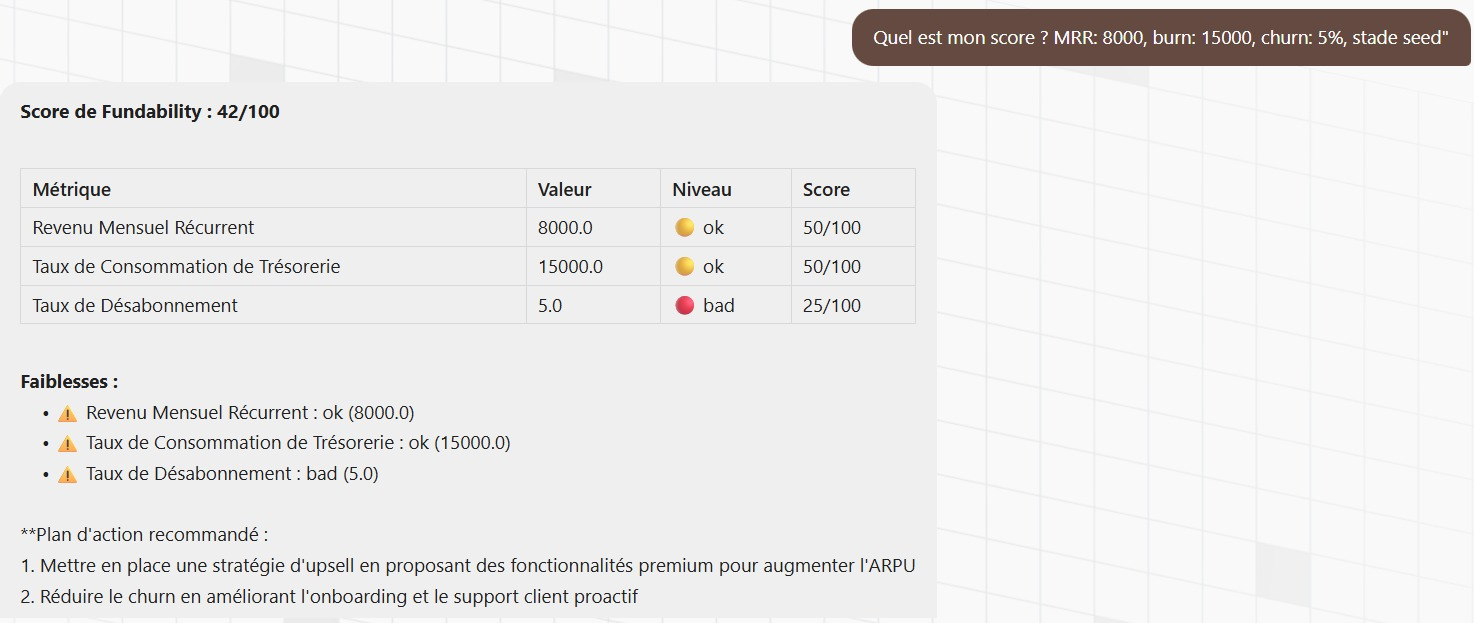
\includegraphics[width=0.92\textwidth]{images/screenshots/scoring_result.jpeg}
\caption{Scénario~1 --- scoring de \textit{fundability}. Requête~: \textit{\og Quel est mon score~? MRR~: 8000, burn~: 15000, churn~: 5\%, stade seed \fg}. Le module retourne un score pondéré de 42/100, une ventilation par métrique avec pastilles de niveau (\textit{ok}/\textit{bad}), une liste de faiblesses et un plan d'action en deux points.}
\label{fig:scoring_result}
\end{figure}

\begin{figure}[H]
\centering
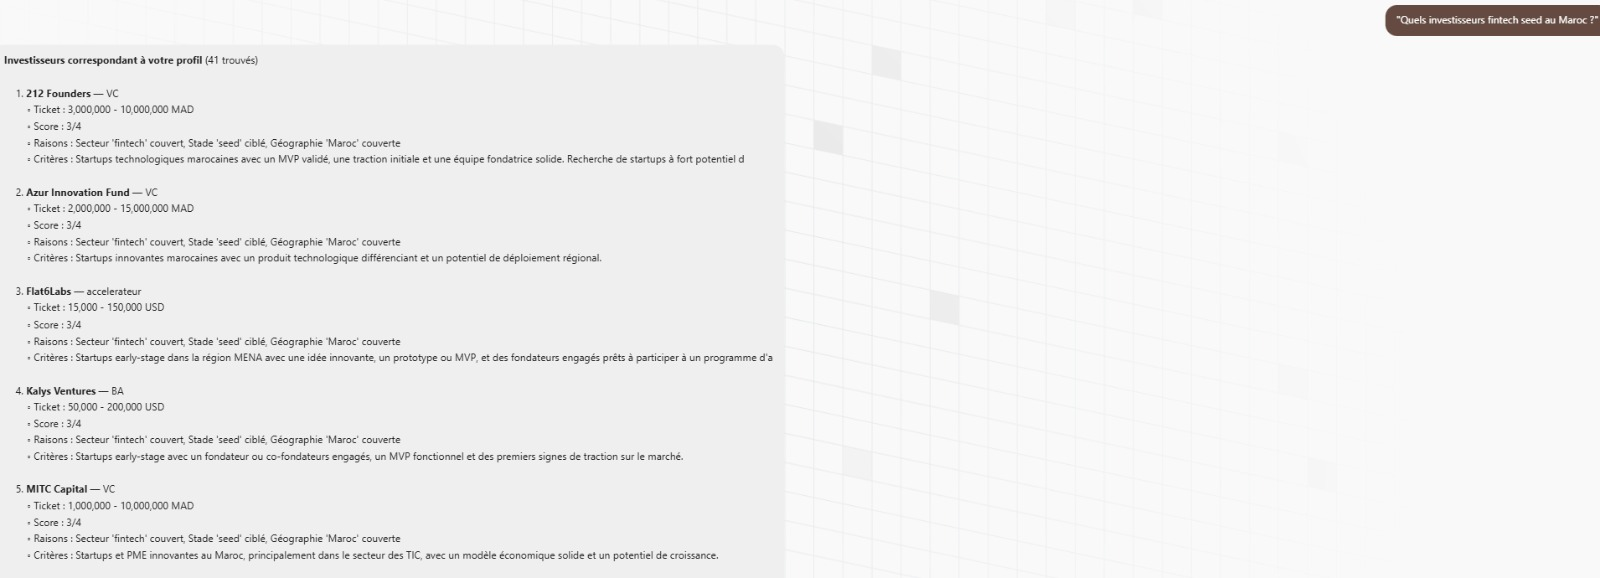
\includegraphics[width=0.92\textwidth]{images/screenshots/investor_matching.jpeg}
\caption{Scénario~3 --- matching investisseurs. Profil saisi~: \textit{fintech, seed, Maroc}. Le module identifie 41 investisseurs du dataset et restitue les cinq premiers (212~Founders, Azur Innovation Fund, Flat6Labs, Kalys Ventures, MITC Capital) avec \textit{ticket}, score de \textit{matching} (3/4 pour tous ici) et raisons détaillées.}
\label{fig:investor_matching}
\end{figure}

\begin{figure}[H]
\centering
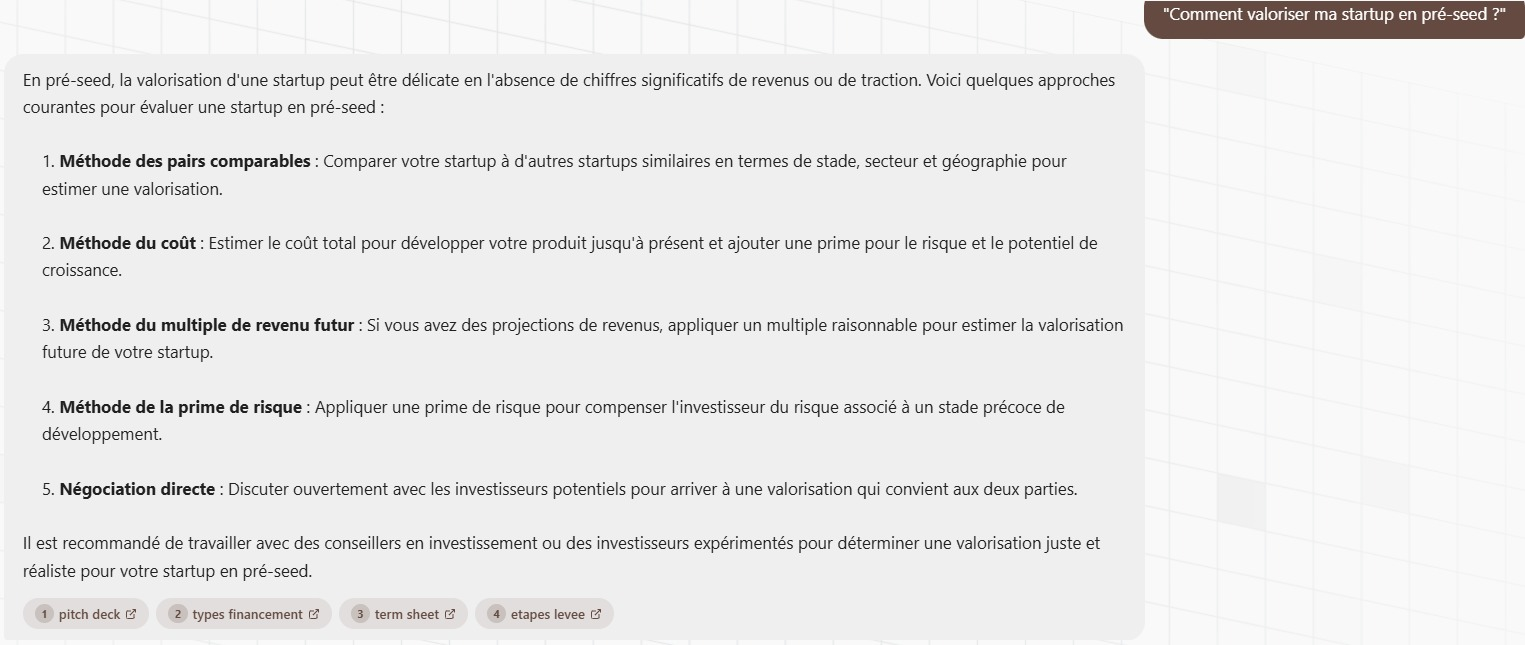
\includegraphics[width=0.92\textwidth]{images/screenshots/qa_rag.jpeg}
\caption{Scénario~6 --- Q\&A \ac{RAG}. Question~: \textit{\og Comment valoriser ma startup en pré-seed~? \fg}. La réponse, générée en \textit{streaming}, présente cinq méthodes de valorisation tirées du guide de \textit{fundraising} du dataset. Les quatre pastilles numérotées en bas (\textit{pitch deck}, \textit{types financement}, \textit{term sheet}, \textit{etapes levee}) sont les sources cliquables attribuées par le moteur de \textit{retrieval}.}
\label{fig:qa_rag}
\end{figure}


\section{Validation du routeur d'intentions}

Le routeur d'intentions est le premier composant sollicité à chaque requête utilisateur. Il distingue quatre classes principales (\code{qa}, \code{scoring}, \code{investors}, \code{grants}) et redirige ensuite la requête vers le module métier approprié. Une erreur à ce niveau se propage donc directement sur la réponse finale, ce qui justifie une validation séparée.

La matrice de confusion a été évaluée sur 200 requêtes représentatives, soit 50 requêtes par classe. Le résultat global est une \textbf{accuracy d'environ 95\%}, avec une diagonale dominante et environ dix requêtes mal classées (figure~\ref{fig:router_confusion}). Les erreurs restantes concernent principalement des formulations ambiguës qui mélangent deux intentions, par exemple une demande évoquant simultanément les subventions et les investisseurs au Maroc.

\begin{figure}[H]
\centering
\includegraphics[page=2,width=0.92\textwidth]{chapters/tamwil_ai_validation.pdf}
\caption{Matrice de confusion du routeur d'intentions, évaluée sur 200 requêtes représentatives.}
\label{fig:router_confusion}
\end{figure}

\begin{table}[H]
\centering
\caption{Synthèse de validation du routeur d'intentions.}
\label{tab:router_validation}
\begin{tabularx}{\textwidth}{@{}l X@{}}
\toprule
\textbf{Critère} & \textbf{Résultat} \\
\midrule
Classes évaluées & \code{qa}, \code{scoring}, \code{investors}, \code{grants} \\
Jeu de test & 200 requêtes représentatives, équilibrées à 50 requêtes par classe \\
Accuracy globale & 190/200 requêtes correctes, soit 95\% \\
F1-score moyen & 95\%, moyenne des quatre classes \\
Erreurs observées & 10 confusions, surtout sur des requêtes multi-intentions ou ambiguës \\
Conclusion & L'approche par mots-clés et \textit{regex} est suffisante pour le périmètre fermé du projet, tout en restant transparente et maintenable \\
\bottomrule
\end{tabularx}
\end{table}

Le détail par classe confirme que la performance n'est pas portée par une seule intention dominante. Les quatre classes obtiennent des scores proches, avec un F1-score compris entre 94,0\% et 96,0\% (tableau~\ref{tab:router_metrics}).

\begin{table}[H]
\centering
\caption{Métriques de classification par classe pour le routeur.}
\label{tab:router_metrics}
\begin{tabularx}{\textwidth}{@{}l c c c c@{}}
\toprule
\textbf{Classe} & \textbf{Vrais positifs} & \textbf{Précision} & \textbf{Recall} & \textbf{F1-score} \\
\midrule
\code{qa}        & 47/50  & 97,9\% & 94,0\% & 95,9\% \\
\code{scoring}   & 48/50  & 96,0\% & 96,0\% & 96,0\% \\
\code{investors} & 48/50  & 92,3\% & 96,0\% & 94,1\% \\
\code{grants}    & 47/50  & 94,0\% & 94,0\% & 94,0\% \\
\textbf{Moyenne} & 190/200 & 95,0\% & 95,0\% & 95,0\% \\
\bottomrule
\end{tabularx}
\end{table}

\begin{figure}[H]
\centering
\includegraphics[page=1,width=0.92\textwidth]{chapters/router_metrics.pdf}
\caption{Synthèse visuelle des métriques du routeur~: accuracy, F1-score moyen, erreurs totales et détail par classe.}
\label{fig:router_metrics_pdf}
\end{figure}

Les métriques utilisent les formules classiques de classification~: précision $= TP/(TP+FP)$, recall $= TP/(TP+FN)$ et F1-score $= 2 \times (\text{précision} \times \text{recall})/(\text{précision}+\text{recall})$. Ce résultat justifie le choix d'un routeur déterministe dans la version actuelle. Un classifieur supervisé de type BERT ou un routeur par \ac{LLM} pourrait améliorer la robustesse sur des formulations plus éloignées des motifs prévus, mais nécessiterait un dataset annoté plus large.

\section{Tests du pipeline RAG}

Les cinq sous-étapes du pipeline ont été validées indépendamment.

\paragraph{Ingestion.} Le module \code{data\_loader.py} a été exécuté en \textit{standalone} et charge les six sources sans erreur (tableau~\ref{tab:ingestion}).

\begin{table}[H]
\centering
\caption{Résultats de l'ingestion sur le dataset cible.}
\label{tab:ingestion}
\begin{tabularx}{\textwidth}{@{}l X c@{}}
\toprule
\textbf{Source} & \textbf{Résultat} & \textbf{Statut} \\
\midrule
Investisseurs        & 41 profils chargés et validés & \textbf{OK} \\
Subventions          & 25 programmes chargés et validés & \textbf{OK} \\
Métriques            & 18 \ac{KPI} chargés et validés & \textbf{OK} \\
\ac{FAQ}             & 54 Q\&A chargés et validés & \textbf{OK} \\
Guides fundraising   & 6 fichiers Markdown chargés & \textbf{OK} \\
Régulations          & 4 fichiers Markdown chargés & \textbf{OK} \\
\bottomrule
\end{tabularx}
\end{table}

\paragraph{Chunking.} L'exécution d'\code{ingest.py} produit environ 250 vecteurs indexés dans ChromaDB pour l'ensemble du dataset, avec préservation des métadonnées (\code{source}, \code{type}). Les paramètres utilisés (\code{chunk\_size~=~500}, \code{overlap~=~50}) offrent un compromis correct entre taille de contexte injectable au \ac{LLM} et granularité du \textit{retrieval}.

\paragraph{Embeddings.} Le modèle \texttt{paraphrase-multilingual-MiniLM-L12-v2} produit des vecteurs de 384 dimensions. Des tests qualitatifs sur une trentaine de requêtes françaises couvrant les six intentions du routeur confirment la pertinence des \textit{embeddings} (scores de similarité élevés sur les passages attendus, faibles sur les passages non pertinents).

\paragraph{Base vectorielle.} ChromaDB a été construit et persisté. La mesure effectuée à date donne \textbf{9,4~MB} pour l'ensemble \code{chroma\_db/}. Le chargement depuis le disque est quasi instantané (\textit{warm start} inférieur à une seconde), ce qui justifie de ne pas reconstruire l'index à chaque démarrage du serveur.

\paragraph{Retriever.} La recherche par similarité cosinus a été testée sur les scénarios fonctionnels ainsi que sur des requêtes délibérément bruitées (fautes d'orthographe, mélange français-anglais)~; les résultats restent pertinents grâce à la robustesse du modèle multilingue.


\subsection{Optimisation de Recall@K}

Le paramètre $K$ détermine le nombre de \textit{chunks} récupérés puis injectés dans le contexte du \ac{LLM}. Un $K$ trop faible prive le modèle d'informations utiles, tandis qu'un $K$ trop élevé augmente le contexte, la latence et le coût en tokens. La validation du pipeline a donc mesuré le rappel documentaire pour plusieurs valeurs de $K$ (tableau~\ref{tab:recall_k}).

\begin{table}[H]
\centering
\caption{Recall@K du pipeline \ac{RAG} sur la base ChromaDB.}
\label{tab:recall_k}
\begin{tabularx}{\textwidth}{@{}c c l X@{}}
\toprule
\textbf{K} & \textbf{Recall} & \textbf{Verdict} & \textbf{Interprétation} \\
\midrule
1  & 55\% & Insuffisant & De nombreuses informations pertinentes ne sont pas récupérées. \\
3  & 78\% & Acceptable & Niveau correct pour des questions simples, mais fragile sur des sujets complexes. \\
5  & 92\% & Optimal & Meilleur compromis entre couverture documentaire, latence et coût. \\
10 & 95\% & Rendement décroissant & Gain limité à +3 points pour un contexte deux fois plus large. \\
\bottomrule
\end{tabularx}
\end{table}

La figure~\ref{fig:recall_k_pdf} visualise cette progression et montre le rendement décroissant après $K=5$. Le choix opérationnel est donc \code{TOP\_K=5}. Le passage de $K=5$ à $K=10$ améliore le rappel de 92\% à 95\%, mais double le volume de contexte envoyé au modèle. Ce surcoût n'apporte pas d'amélioration perceptible de la réponse finale dans les scénarios testés.

\begin{figure}[H]
\centering
\includegraphics[page=3,width=0.92\textwidth]{chapters/tamwil_ai_validation.pdf}
\caption{Recall@K du pipeline \ac{RAG} pour $K=1,3,5,10$.}
\label{fig:recall_k_pdf}
\end{figure}

\section{Performance de l'API de streaming}

L'\ac{API} FastAPI expose les réponses via \ac{SSE}, ce qui permet au frontend d'afficher les premiers tokens avant la fin de la génération complète. La métrique suivie est donc le temps jusqu'au premier token reçu par l'interface.

\begin{table}[H]
\centering
\caption{Distribution des latences mesurées sur 100 requêtes.}
\label{tab:latency}
\begin{tabularx}{\textwidth}{@{}l c X@{}}
\toprule
\textbf{Métrique} & \textbf{Valeur} & \textbf{Interprétation} \\
\midrule
Latence médiane p50 & ${\sim}220$~ms & Premier token perçu quasi instantanément par l'utilisateur. \\
Latence p95 & ${\sim}450$~ms & Seuil haut observé sur les requêtes plus coûteuses. \\
Maximum observé & ${\sim}600$~ms & Longue traîne liée surtout aux requêtes \ac{RAG} avec recherche vectorielle préalable. \\
\bottomrule
\end{tabularx}
\end{table}

La distribution complète est représentée dans la figure~\ref{fig:latency_pdf}. Les requêtes dépassant 400~ms correspondent principalement aux questions ouvertes qui déclenchent la récupération de $K=5$ passages dans ChromaDB avant l'appel au \ac{LLM}. Le \textit{streaming} \ac{SSE} rend toutefois cette latence acceptable, car l'utilisateur voit la réponse se construire progressivement au lieu d'attendre un bloc complet.

\begin{figure}[H]
\centering
\includegraphics[page=4,width=0.92\textwidth]{chapters/tamwil_ai_validation.pdf}
\caption{Distribution des latences de l'\ac{API} en \textit{streaming}, mesurée sur 100 requêtes.}
\label{fig:latency_pdf}
\end{figure}

\subsection{Choix de GPT-3.5}

Le choix de GPT-3.5 via \ac{API} est cohérent avec la contrainte d'expérience utilisateur~: maintenir un \textit{streaming} fluide et un premier token autour de 220~ms. Un modèle local de taille comparable exécuté sur processeur aurait des latences sensiblement supérieures sans \ac{GPU} dédié. La migration vers un modèle local reste pertinente en production pour réduire les coûts, mais elle devra être arbitrée avec les exigences de latence.

\section{Tests unitaires}

Six fichiers de tests unitaires couvrent l'ensemble des modules (tableau~\ref{tab:unit_tests}). La suite se lance avec \code{pytest} depuis la racine du dépôt.

\begin{table}[H]
\centering
\caption{Fichiers de tests unitaires et périmètre couvert.}
\label{tab:unit_tests}
\begin{tabularx}{\textwidth}{@{}l l X@{}}
\toprule
\textbf{Fichier} & \textbf{Module testé} & \textbf{Périmètre} \\
\midrule
\code{test\_scoring.py}             & \code{scoring.py}             & classification, calcul pondéré, métriques inversées \\
\code{test\_diagnostic.py}          & \code{diagnostic.py}          & analyse par \ac{KPI}, génération de résumé \\
\code{test\_matching\_investors.py} & \code{matching\_investors.py} & score de \textit{matching}, tri, filtrage multi-critère \\
\code{test\_matching\_grants.py}    & \code{matching\_grants.py}    & éligibilité pays/stade/secteur/âge, \textit{wildcard} \\
\code{test\_router.py}              & \code{router.py}              & détection d'intention, extraction \textit{regex}, \textit{fallback} \\
\code{test\_rag.py}                 & \code{rag\_qa.py}, \code{retriever.py} & \textit{retrieval}, enrichissement de requête \\
\bottomrule
\end{tabularx}
\end{table}

Les tests d'intégration \textit{end-to-end} (frontend $\to$ backend $\to$ \ac{LLM}) ne sont pas couverts dans la version actuelle~; ils figurent dans les perspectives au chapitre suivant.

\section{Discussion et limites}

\subsection{Points forts}

\begin{itemize}
  \item Le pipeline \ac{RAG} fonctionne de bout en bout en français, avec des résultats pertinents sur les six scénarios.
  \item La validation quantitative donne ${\sim}95\%$ d'accuracy pour le routeur, 92\% de Recall@5 pour le \ac{RAG}, et un premier token médian autour de 220~ms.
  \item Les \textit{embeddings} multilingues locaux offrent un bon rapport qualité/coût~: aucun appel \ac{API} facturé pour la vectorisation.
  \item ChromaDB persistant autorise un démarrage rapide du serveur (pas de réindexation).
  \item L'architecture modulaire facilite les tests et les évolutions futures.
  \item Le dataset, bien que modeste en volume, est original et adapté au contexte marocain.
  \item Le \textit{streaming} \ac{SSE} offre une expérience utilisateur comparable aux assistants conversationnels grand public.
  \item La détection de \textit{greetings} économise des appels \ac{API} inutiles.
  \item Le mode \textit{fallback} garantit une dégradation gracieuse lorsque l'\ac{API} OpenAI n'est pas disponible.
\end{itemize}

\subsection{Limites identifiées}

\begin{itemize}
  \item Le dataset (${\sim}504$~KB) est relativement petit et gagnerait à être enrichi, en particulier sur les investisseurs régionaux africains et sur les subventions sectorielles.
  \item Le \ac{LLM} utilisé (\textit{GPT-3.5-turbo}) est le moins coûteux de la gamme OpenAI~; une migration vers un modèle plus récent améliorerait la qualité de la génération au prix d'un coût \ac{API} supérieur.
  \item La détection d'intention par mots-clés et \textit{regex} atteint environ 95\% d'accuracy sur le jeu de validation, mais peut encore échouer sur des formulations inhabituelles ou multi-intentions~; une classification par \ac{LLM} serait plus robuste.
  \item Le \ac{CORS} est limité à \code{localhost:3000}~; une configuration spécifique sera nécessaire pour un déploiement en ligne.
  \item L'historique des conversations est stocké uniquement côté client (\code{localStorage}), ce qui empêche de retrouver ses conversations depuis un autre navigateur ou un autre appareil.
  \item Les tests d'intégration \textit{end-to-end} ne sont pas automatisés~; seuls les tests unitaires, les mesures composant par composant et la validation manuelle des scénarios fonctionnels sont en place.
\end{itemize}

\begin{callout}
En synthèse, \tamwil{} est opérationnel pour un usage en local ou sur un environnement de démonstration. Chaque composant critique a été évalué indépendamment~: routeur d'intentions, \textit{retrieval} \ac{RAG} et \ac{API} de \textit{streaming}. Les limites identifiées concernent principalement les aspects de scalabilité (dataset, persistance serveur, déploiement) et de finition (intent-detection, suite de tests), et sont discutées plus en détail dans les perspectives.
\end{callout}
